This chapter summarises and reflects upon the project as a whole, discussing the various aspects that went well and those that can be improved. The initial project aims defined in the Introduction in Section \ref{sec:introduction-project-aims} are first reviewed, followed by the future work for the project. Finally, the chapter concludes with an analysis of the limitations of the current project and a future commercial application before ending with general reflections about what was accomplished and learned through this project.

%%%%%%%%%%%%%%%%%%%%%%%%%%%%%%%%%%%%%%%%%%%%%%%%%%%%%%%%%%%%%%%%%%%%
%%%%%%%%%%%%%%%%%%%%%%%%%%%%%%%%%%%%%%%%%%%%%%%%%%%%%%%%%%%%%%%%%%%%
%%%%%%%%%%%%%%%%%%%%%%%%%%%%%%%%%%%%%%%%%%%%%%%%%%%%%%%%%%%%%%%%%%%%

\section{Achievements}

The main goal of this project was to design and implement a prototype system to tackle the problem of exponential unstructured data growth in the form of a content-based video retrieval system oriented towards matching mobile-recorded video queries to a movie. After investigating a wide array of potential feature extraction and comparison methods to combine in order to come up with a unique solution, a functional system divided into three phases was created. The first phase processed the videos in the databases to generate compact signatures by extracting colour features and storing them in histograms. The second phase repeated the process with an input query video that is matched to one of the database videos by calculating the distances between the videos' compact signatures. Finally, the third phase was dedicated to make the system suitable for movies by segmenting the videos in the database through a shot boundary detection algorithm.\\

This pipeline of three phases that constituted the system produced positive results with a custom database of 50 videos ranging from 7 to 14 seconds. Indeed, it accurately found the correct matches to queries recorded with a mobile device that included undesired camera movement and poor framing (recorded at a distance and at an angle from the screen) with accuracies reaching a maximum of 93.18\%. However, the system fell short when dealing with unfavourable environment conditions such as the non-white light sources in dark environments and light reflections glaring on the screen, with a minimum of 45.45\% accuracy and in some extreme cases, mismatches.\\

Unfortunately, the system could not be tested with a database of movies due to availability and licensing constraints, but a single movie was used to test the database pre-processing phase of the system. The movie was reduced to less than 1\% of its original size thanks to the shot boundary detection algorithm, which could be used as one of the database video in the two other phases, thus showing the links between the pipeline phases. Overall, almost every aim originally set in Section \ref{sec:introduction-project-aims} was achieved, with the exception of testing the system with a database of movies and creating a true link between the database pre-processing and the offline feature extraction phases which was only conceptualised.
    
%%%%%%%%%%%%%%%%%%%%%%%%%%%%%%%%%%%%%%%%%%%%%%%%%%%%%%%%%%%%%%%%%%%%
%%%%%%%%%%%%%%%%%%%%%%%%%%%%%%%%%%%%%%%%%%%%%%%%%%%%%%%%%%%%%%%%%%%%
%%%%%%%%%%%%%%%%%%%%%%%%%%%%%%%%%%%%%%%%%%%%%%%%%%%%%%%%%%%%%%%%%%%%

\section{Future Work}

A lot of improvements can be made to the system in its current state to improve the runtime and accuracy in order to ultimately use larger databases and longer videos.

\subsection{Current Pipeline Improvements}

Multiple improvements could be accomplished without modifying the original system's design. The first change involves the histograms. Rather than generating averaged global histograms for each shot, region-based histograms should be generated instead. For example, the frames used to generate the histograms can be divided into a number of regions, and an average histogram could be generated for each region. This would ensure a much higher level of accuracy when matching the query video to a database video as the histograms no longer describe the colour distribution throughout the entire image but for a smaller localised region. For example, if the two frames contain both 40\% of blue, where one corresponds to the sky and one to the sea, then a global histogram would not be able to differentiate the two frames easily, whereas a region-based histogram would as the the blues would not be in the same region. An illustration of a frame segmented into five distinct regions can be found in Figure \ref{fig:conclusions-image_regions}.

\begin{figure}[h] 
\centerline{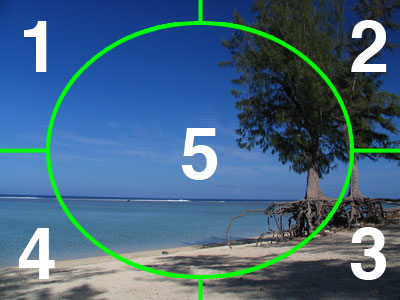
\includegraphics[width=0.5\textwidth]{figures/conclusions/image_regions.jpg}}
\caption{\label{fig:conclusions-image_regions}Example of a frame segmented into 5 regions.}
\end{figure}

Additionally, histogram models that do not produce accurate results, such as the greyscale and RGB histograms, could be excluded from future versions to only include HSV histograms and histograms with similar levels of complexity such as HSL\footnote{Hue Saturation Lightness} histograms. A system generating HSV and HSL histograms only while excluding greyscale and RGB histograms would compute results with much higher accuracies. Indeed, considering the queries used in Chapter \ref{ch:chapter6}, 

\subsection{Automatic Query Processing}

Automatic ROI selection (detect screen edges with edge and corner detector algorithms)

\subsection{Interface-Related Improvements}

In terms of interface, simple changes can be carried out to make the system more usable, without the need to create a marketable mobile application yet. The first change is the interface itself, replacing the CLI with a GUI. A GUI would allow the results to be displayed more easily on the screen along with simpler interaction through button presses rather than console argument parsing. The generated data, such as the matched video, the histograms and the results tables would be more easily accessible and readable. Improving the system to a GUI could be done using either TKinter, the native GUI library for Python, if Python remains the programming language used, or by rendering a clean HTML webpage.

improve ROI selection to take 4 points rather than 2 (will increase accuracy for query videos that are at an angle, not filming the screen from a straight point of view)

\subsection{System Redesign for Large-Scale Databases}

change learning model: deep learning. Mention that with improvements, could have worked with small database of movies rather than short videos

% \begin{itemize}
%     \item more features to complement the colour-based features (e.g. motion and shape features) and improve the accuracy
%     \item make use of sound to further improve accuracy
% \end{itemize} 
% 

%%%%%%%%%%%%%%%%%%%%%%%%%%%%%%%%%%%%%%%%%%%%%%%%%%%%%%%%%%%%%%%%%%%%
%%%%%%%%%%%%%%%%%%%%%%%%%%%%%%%%%%%%%%%%%%%%%%%%%%%%%%%%%%%%%%%%%%%%
%%%%%%%%%%%%%%%%%%%%%%%%%%%%%%%%%%%%%%%%%%%%%%%%%%%%%%%%%%%%%%%%%%%%

\section{Limitations}

\subsection{Project Limitation}

the time constraints of this project

\subsection{Commercial Application Limitations}

The main limitations of a future marketable application to match movies lie within the nature of the data itself. Indeed, videos, and in particular movies, are very large objects. No matter the efficiency of the algorithm, processing them requires a lot of time and computing power, which is not always available. This fact is verified with the evaluation test carried out in Section \ref{sec:evaluation-movie-segmentation-test}, where pre-processing a single feature-length movie took an average of 2 hours and 35 minutes. This step includes the actual visual content extraction to represent a movie with features. Given a database of at least 100,000 movies, which would be a realistic number to start a commercial movie matching application, the amount of time to pre-process and later train the model would simply be colossal and unrealistic nowadays. Additionally, 

% limitations of working with large database of movies:
% \begin{itemize}
%     \item too much data to process, could perhaps be pre-processed in advance
%     \item copyright issues of having all these movies
% \end{itemize}
    
%%%%%%%%%%%%%%%%%%%%%%%%%%%%%%%%%%%%%%%%%%%%%%%%%%%%%%%%%%%%%%%%%%%%
%%%%%%%%%%%%%%%%%%%%%%%%%%%%%%%%%%%%%%%%%%%%%%%%%%%%%%%%%%%%%%%%%%%%
%%%%%%%%%%%%%%%%%%%%%%%%%%%%%%%%%%%%%%%%%%%%%%%%%%%%%%%%%%%%%%%%%%%%

\section{Project Summary \& Reflections}

todo\\

The code developed for this dissertation can be found online at the following URL: \url{https://github.com/Adamouization/Content-Based-Video-Retrieval-Code}.